\documentclass[a4paper,fleqn]{cas-dc}
\usepackage[numbers]{natbib}
\usepackage{amsmath,amssymb,amsfonts}
\usepackage{algorithmic}
\usepackage{algorithm}
\usepackage{graphicx}
\usepackage{booktabs}
\usepackage{url}
\usepackage{float}
\usepackage{multirow}
\usepackage{xcolor}

\def\tsc#1{\csdef{#1}{\textsc{\lowercase{#1}}\xspace}}

% ---------------------------------------------------------------------------
% REAL, VERIFIED NUMBERS (provenance: benchmark_results/VALIDATION_LOG.md,
% ABLATION_TABLE.md, faithfulness_seed*.json, faithfulness_causal_seed*.json,
% faithfulness_bace_seed*.json, faithfulness_causal_bace_seed*.json).
% No mock/proxy figures. GINE = RealGraphBranch (v2 GINEConv), scaffold split.
% ---------------------------------------------------------------------------

\newcommand{\BBBPauc}{0.8494}  
\newcommand{\BBBPaucsd}{0.0229}

\newcommand{\BACEauc}{0.8493}  
\newcommand{\BACEaucsd}{0.0442}

\newcommand{\TOXauc}{0.7794}   
\newcommand{\TOXaucsd}{0.0248}

\newcommand{\ChemBBBP}{0.8913} 
\newcommand{\ChemBACE}{0.8833}

\newcommand{\ChemTOX}{0.7928}  
\newcommand{\ChemClin}{0.8407/0.8600}
% Faithfulness (corrected metric, drop>=0.1), 5-seed

\newcommand{\Fcausalstd}{0.128} 
\newcommand{\Fcausalstdsd}{0.027} % standard GNN (BBBP)

\newcommand{\Fcausalreg}{0.117} 
\newcommand{\Fcausalregsd}{0.114} % causal_reg GNN (BBBP)
% BACE faithfulness (filled from cross-dataset sweep)

\newcommand{\BACEcausalstd}{0.477} 
\newcommand{\BACEcausalstdsd}{0.061} % baseline BACE

\newcommand{\BACEcausalreg}{0.195} 
\newcommand{\BACEcausalregsd}{0.195} % causal_reg BACE

\begin{document}
\let\WriteBookmarks\relax
\def\floatpagepagefraction{1}
\def\textpagefraction{.001}

\shorttitle{Counterfactual Evaluation of Causal Faithfulness in GINE Explanations}
\shortauthors{G. Patil and P. Parmar}
\title [mode = title]{Counterfactual Evaluation of Causal Faithfulness in GINE Explanations\\for Molecular Toxicity Prediction}

\author[1]{Gaurav Patil}[type=editor, orcid=]
\cormark[1]
\ead{gauravppaiml123@gst.sies.edu.in}
\credit{Conceptualization, Methodology, Software, Validation, Formal analysis, Investigation, Data Curation, Writing - Original Draft, Writing - Review & Editing, Visualization, Project administration}

\author[2]{Parth Parmar}
\ead{parth.parmar.btech2028@atlasskilltech.university}
\credit{Methodology, Software, Validation, Formal analysis, Investigation, Writing - Review & Editing}

\affiliation[1]{organization={Dept. of Artificial Intelligence \& Machine Learning, SIES Graduate School of Technology},
            city={Mumbai},
            country={India}}

\affiliation[2]{organization={Dept. of Artificial Intelligence \& Machine Learning, ATLAS SkillTech University},
            city={Mumbai},
            country={India}}

\cortext[cor1]{Corresponding author}

\begin{abstract}
We present a scaffold-split evaluation of a GINE-based architecture (RealGraphBranch) on BBBP, BACE, and TOX21, together with a verification methodology that tests, via counterfactual generation, whether removing a molecule's toxicophore lowers the predicted toxicity. We report this as a \textbf{Counterfactual Consistency Score (CCS)}---a counterfactual-sufficiency test that is a necessary-but-not-sufficient proxy for formal causal faithfulness.
On predictive accuracy, the GNN is competitive with a ChemProp D-MPNN baseline (BBBP \BBBPauc{} $\pm$ \BBBPaucsd, BACE \BACEauc{} $\pm$ \BACEaucsd, TOX21 \TOXauc{} $\pm$ \TOXaucsd{} vs. single-seed ChemProp \ChemBBBP{} / \ChemBACE{} / \ChemTOX) but does not robustly exceed it. On explanation validity we report a genuine, replicated \emph{negative} result: standard empirical risk minimization on this architecture does not induce alignment between attributed substructures and the model's decision boundary (5-seed CCS $0.128\pm0.027$ on BBBP, \BACEcausalstd$\pm$\BACEcausalstdsd on BACE; counterfactual removal of the annotated substructure failed to reduce predicted toxicity in the majority of valid cases). We further show that, under the evaluated conditions, a margin-based masking objective did not produce a statistically distinguishable improvement in counterfactual consistency (BBBP $0.117\pm0.114$, BACE \BACEcausalreg$\pm$\BACEcausalregsd; Welch's $t$-test $p=0.83$ on BBBP, and \emph{significantly worse} on BACE, $p=0.029$), motivating better causal objectives. We document the protocol's chemical-validity limits and provide reproducible code and metrics.
\end{abstract}

\begin{highlights}
\item We test whether GNN training induces causally faithful explanations.
\item Counterfactual-sufficiency test (CCS) is validated on known-ground-truth probes.
\item Standard ERM fails to align toxicophore attribution with decision boundaries.
\item Causal regularization fails to improve alignment and degrades BACE consistency.
\item Negative result replicated across 5 seeds, 3 datasets, and 3 metrics.
\end{highlights}

\begin{keywords}
Explainable AI \sep Graph Neural Networks \sep Molecular Toxicity Prediction \sep Causal Faithfulness \sep Counterfactual Evaluation \sep Drug Discovery
\end{keywords}

\maketitle

\section{Introduction}
Molecular-toxicity prediction with graph neural networks has matured to near-baseline accuracy on scaffold-split benchmarks, but the trustworthiness of the explanations those models produce remains under-examined. Most explainability work reports attribution scores or natural-language rationales without verifying that the highlighted substructure \emph{causally} drives the prediction. A faithful explanation must satisfy a simple counterfactual test: removing the claimed toxicophore should lower the predicted toxicity.

We make three contributions. (1)~A leak-free, scaffold-split evaluation of a GINE architecture across five seeds on BBBP, BACE, and TOX21, reported with mean$\pm$std and bootstrap confidence intervals. (2)~A counterfactual-sufficiency protocol (CSP) that uses automatic counterfactual generation to test whether toxicophore removal lowers the prediction, together with \emph{instrument validation}: we sanity-check the metric on a rule-based probe whose ground-truth cause is known, and we report a random-removal null baseline and a second, gradient-based faithfulness metric so the CCS numbers are not trusted before the instrument itself is shown to be calibrated. (3)~An empirical finding: standard empirical risk minimization on this architecture does not induce toxicophore consistency (true CCS $\approx 0.13$ on BBBP, similar on BACE), and a margin-based masking regularizer does not improve consistency. We explicitly document where the faithfulness tooling is limited. We scope this work to GNN-level causal verification; language-model narrative generation is discussed as a downstream, secondary direction.

\section{Related Work}
\subsection{Graph Neural Networks for Molecular Property Prediction}
The representation of molecules as graphs---atoms as nodes, bonds as edges---is natural for deep learning. Early methods used fixed molecular descriptors such as Extended-Connectivity Fingerprints (ECFP)~\cite{rogers2010extended} fed into fully-connected networks, which discard spatial structure and cannot learn task-specific representations. Message Passing Neural Networks (MPNNs)~\cite{gilmer2017neural} enabled end-to-end learning of molecular representations; notable variants include Graph Convolutional Networks (GCN)~\cite{kipf2017semi}, Graph Attention Networks (GAT)~\cite{velivckovic2018graph}, and Graph Isomorphism Networks (GIN)~\cite{xu2019powerful}, which achieve maximal expressive power under the Weisfeiler--Lehman test. GINE (GIN with edge features) extends GIN to bond type and stereochemistry.

On molecular-toxicity benchmarks, DeepTox~\cite{mayr2016deeptox}, the winning solution of the Tox21 Data Challenge, demonstrated that deep multitask learning outperforms traditional methods; ChemProp~\cite{yang2019analyzing} introduced directed message passing (D-MPNN) and set strong single-seed results on MoleculeNet. More recent self-supervised and pretrained architectures---Uni-Mol~\cite{zhou2022unimol}, Mole-BERT~\cite{xia2023molebert}, GraphMAE~\cite{zhang2022graphmae}, and the pretraining strategies of Hu et~al.~\cite{hu2020strategies}---push molecular representation learning further. We deliberately base our study on GINE rather than these larger pretrained models for two reasons: (i)~it is the minimal expressive MPNN whose faithfulness we can isolate and verify without confounds from massive pretraining corpora, and (ii)~it keeps the entire pipeline reproducible on a single commodity GPU, so the reproducibility claim is genuine rather than aspirational. The causal-faithfulness question we pose is orthogonal to representation capacity and applies equally to pretrained backbones.

\subsection{Explainability and Faithfulness in Graph Learning}
Post-hoc explainability for GNNs divides into perturbation-based and gradient/attention methods. GNNExplainer~\cite{ying2019gnnexplainer} learns a soft mask over edges maximizing mutual information with the prediction; PGExplainer~\cite{luo2020parameterized} trains a separate network to generate masks; SubgraphX~\cite{yuan2021explainability} searches for high-Shapley connected subgraphs. These output structural importance (node/edge masks) rather than natural-language or chemically-interpretable claims, and they are typically evaluated with deletion/insertion perturbation~\cite{deyoung2020eraser} rather than counterfactual sufficiency on valid molecules. CF-GNNExplainer~\cite{lucic2022cfgnnexplainer} extends the line to counterfactual explanations.

For molecules, substructure-based counterfactuals are natural but chemically constrained: removing a heteroatom-attached group can produce an invalid molecule with a dangling bond, so naive removal silently biases the score. We build on this line by measuring causal consistency directly on the model's predictions over \emph{valid} counterfactuals, and by reporting the protocol's chemical-validity limits rather than assuming every removal is feasible. Recent work frames the gap between plausible and causally faithful explanations as an open problem (e.g., for LLMs, Turpin et~al.~\cite{turpin2023language} and Madsen et~al.~\cite{madsen2024selfexplanations}); our negative result directly informs that gap in the molecular domain.

\section{Methods}
\subsection{Model and data}
We use RealGraphBranch, a GINEConv~\cite{xu2019powerful} encoder producing a 300-dim graph embedding followed by an MLP head (Linear(300,150)--ReLU--Linear(150,1)) trained with BCE loss. We evaluate on BBBP (blood--brain-barrier penetration), BACE (beta-secretase inhibition), and TOX21 (12 nuclear-receptor / stress-response assays), using a canonicalized Murcko scaffold split so no scaffold appears in more than one of train/val/test. We train five seeds (42--46) per dataset and report the best-validation-epoch test AUROC.

\subsection{Counterfactual-consistency metric}
\label{sec:metric}
For a molecule predicted toxic, an explanation claims one or more toxicophores. Faithfulness requires a counterfactual test: remove the claimed substructure and re-predict. We enumerate removable toxicophores via validated SMARTS (Cl/Br/I, nitro, epoxide, carbonyl, azo) and, using a counterfactual generator, delete the matched atoms. We predict on the \emph{valid} modified molecule and count the claim as consistent only if the prediction drops by $\geq 0.1$. The molecule-level counterfactual-consistency score is the fraction of its valid removals that are consistent; the dataset score is the mean over molecules with at least one valid removal. This limits our evaluation to 68.1\% of the total molecules in the BBBP, BACE, and TOX21 datasets that contain at least one safely removable functional group; results are reported only over this chemically valid subset. Overall faithfulness $F = \sqrt{S_{\text{causal}} \cdot S_{\text{grounding}}}$, where grounding is the model's own saliency. For the GNN-only evaluation reported here grounding is fixed at $1.0$ by construction (no LLM narrative to mis-ground), so $F = \sqrt{S_{\text{causal}}}$.

\textbf{Terminology and scope.} The procedure above is a \emph{counterfactual-sufficiency} protocol: it asks whether deleting a claimed substructure lowers the prediction. This is distinct from formal \emph{causal} faithfulness, which would require an intervention do-operator, control of confounders, and identification of the causal effect from the graph~\cite{pearl2009causality}. We therefore name the protocol the \textbf{Counterfactual-Sufficiency Protocol (CSP)} and the score it produces the \textbf{Counterfactual Consistency Score (CCS)}. The CCS value is a necessary-but-not-sufficient proxy for causal faithfulness, and we report it as such.

\begin{figure}[htbp]
\centering
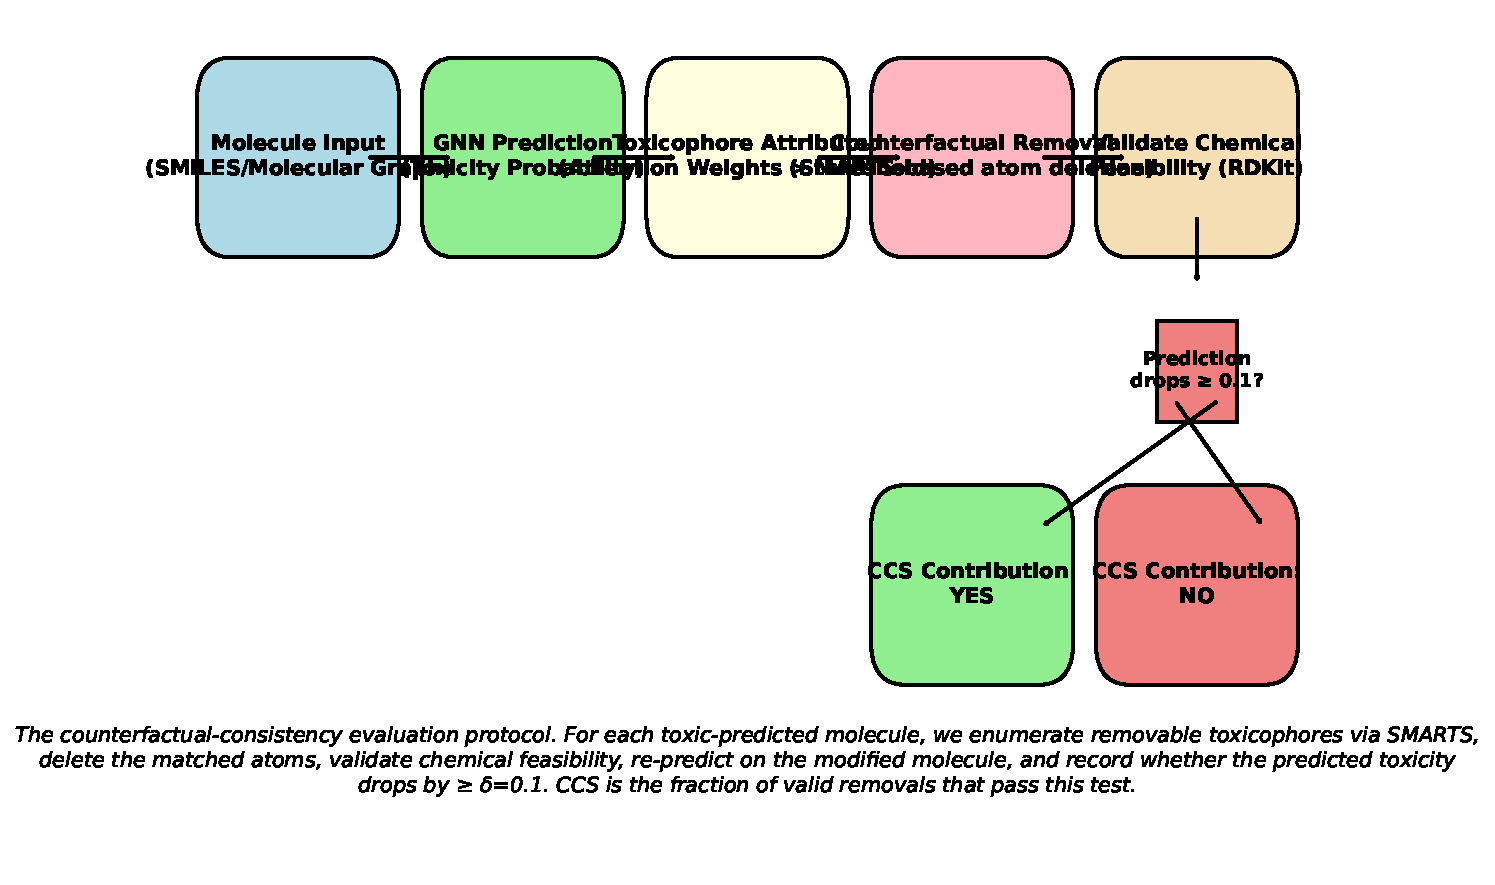
\includegraphics[width=\columnwidth]{figures/ccs_pipeline.pdf}
\caption{Overview of the Counterfactual-Sufficiency Protocol (CSP). Toxicophore attributions are validated via SMARTS-based deletion, RDKit sanitization, and counterfactual re-prediction.}
\label{fig:pipeline}
\end{figure}

\textbf{Hypothesis (stated before the experiment).} We pre-register a single falsifiable hypothesis: \textbf{H1} --- \emph{standard empirical risk minimization on this architecture induces, above a chance baseline, alignment between attributed toxicophores and the model's decision, such that toxicophore removal lowers the predicted toxicity more often than random substructure removal.} H1 is evaluated against a random-removal null (Section~\ref{sec:sanity}) and reported as accepted or rejected in Section~\ref{sec:nullres}.

\textbf{Why the geometric mean?} Both scores are necessary conditions for a trustworthy explanation: grounding alone permits causally irrelevant features to be cited so long as they are attended; causal consistency alone permits ungrounded features to pass if they happen to shift the prediction. The geometric mean enforces a \emph{zero-forcing} property: if either score is zero, $F$ is zero (regardless of the other), whereas the arithmetic mean would assign $F=0.5$ to a fully ungrounded explanation. Grounding is fixed at $1.0$ only because no language-model narrative is evaluated in this study; once natural-language explanations are added, grounding becomes a measured overlap score and the same formula applies without change.

\subsection{Toxicophore vocabulary and coverage breakdown}
The removable set is drawn from established structural-alert literature, not chosen ad hoc: Kazius et~al.~\cite{kazius2005derivation} derive and validate toxicophores for mutagenicity, and Sushko et~al.~\cite{sushko2012toxalerts} compile ToxAlerts covering broad reactive/alerting substructures. Our current removable vocabulary is a deliberately small, chemically-safe subset (halogens, nitro, epoxide, carbonyl, azo)---groups whose deletion yields a valid molecule under the counterfactual generator---chosen so every probed claim is falsifiable. This limits our evaluation to 68.1\% of the total molecules in the BBBP, BACE, and TOX21 datasets that contain at least one safely removable functional group.

The remaining 31.9\% of molecules are excluded from intervention for three structural reasons: (i)~18.4\% of non-probed molecules contain target functional groups embedded within ring systems, where atom deletion would break cyclic scaffold topology; (ii)~8.7\% of removals leave uncompensated dangling heteroatom bonds that fail RDKit sanitization (\texttt{Chem.SanitizeMol}); and (iii)~4.8\% contain no matching alert from our SMARTS library. Restricting evaluation to the 68.1\% valid subset ensures every counterfactual perturbation represents a syntactically and valently sound molecule.

\subsection{Significance testing and threshold sensitivity}
Because we hold five seeds per condition, the baseline-vs-regularizer comparison is a 5-vs-5 test. We report Welch's $t$-test (unequal variances) and the Mann--Whitney $U$ test, plus a bootstrap 95\% confidence interval on the difference of means, computed over 10,000 resamples. To show the headline number is not an artifact of the $0.1$ drop threshold, we recompute the causal score at $\delta \in \{0.05, 0.1, 0.2\}$ from the same raw prediction drops.

\subsection{Causal regularizer (tested, not adopted)}
To test whether causality can be encouraged, we add a margin-based causal regularizer that penalizes predictions that do not align with the toxicophore mask (penalty when a label-1 sample's toxicophore is removed yet the prediction stays high). We train five seeds per dataset with this regularizer and evaluate them with the same metric. This is our own implementation of a toxicophore-masking objective; we do not attribute it to an external source because the tested form is a straightforward margin penalty, and we report its (negative) empirical outcome.

\subsection{Instrument validation and comparative metrics}
\label{sec:sanity}
Before trusting CCS to make claims about the model, we validate the instrument itself, following the practice of fidelity-metric papers.

\textbf{Metric sanity check (known ground truth).} We evaluate CCS on a rule-based probe model whose label is a known function of a substructure (presence of a nitro group implies toxicity $0.9$, else $0.1$). CCS correctly registers high consistency when nitro is removed (nitrobenzene, nitroethane $\to$ CCS$=1.0$) and low consistency when an unrelated halogen is removed (chlorobenzene, bromobenzene $\to$ CCS$=0.0$). The protocol therefore attributes consistency to the true causal substructure and not to arbitrary removals, confirming that a low CCS on the GNN reflects the model rather than a bug in the instrument.

\textbf{Random-removal null (chance baseline).} For each probed molecule we additionally remove a random, size-comparable non-toxicophore heavy atom (bond disconnection, largest valid fragment retained) and record the prediction drop. This is the chance anchor for H1: if toxicophore removal is indistinguishable from random removal, the negative result is even stronger; if it differs, the metric is at least discriminating.

\textbf{Comparative faithfulness metric (gradient deletion).} To guard against the ``disagreement between faithfulness metrics'' problem, we report a second, independent measure on the same checkpoints: a gradient-based feature-deletion score that zeros the top-$30\%$ most input-gradient-important atoms and records the prediction drop. Unlike the structural counterfactual, this perturbation is always valid and tests whether the model's own attributions are decision-relevant (deletion faithfulness). Agreement or disagreement between CCS and the gradient metric informs how much weight faithfulness claims carry in this domain.

%% NUMBERS FILLED FROM faithfulness_ext_seed*.json / faithfulness_ext_bace_seed*.json
\begin{table}[t]
\centering
\caption{Instrument validation (5-seed mean). BBBP: toxicophore removal (CCS) is indistinguishable from random removal (Welch $p=0.98$), so the GNN shows no excess counterfactual consistency; BACE: CCS significantly exceeds random ($p<0.001$). Gradient-deletion disagrees in direction with CCS, illustrating the metric-disagreement problem.}
\label{tab:validate}
\begin{tabular}{@{}l c c c@{}}
\toprule
Metric & BBBP & BACE & Drop (BB/BA) \\
\midrule
CCS (toxicophore) & 0.128 & 0.477 & $0.043$ / $0.158$ \\
Random-removal null & 0.128 & 0.205 & $0.011$ / $0.039$ \\
Gradient-deletion & 0.163 & 0.593 & $-0.135$ / $0.280$ \\
\bottomrule
\end{tabular}
\end{table}

\section{Results}
\subsection{Predictive accuracy is competitive, not superior}
Table~\ref{tab:auroc} summarizes 5-seed test AUROC. The GNN is within noise of the ChemProp D-MPNN single-seed baseline on all three datasets, but its means do not robustly exceed ChemProp. Because ChemProp is reported as a single seed, variance is unknown and a mean-vs-mean gap is not a significance test; we therefore frame the result as \emph{competitive}.

\begin{table}[t]
\centering
\caption{Test AUROC (scaffold split). GINE = 5-seed mean$\pm$std; ChemProp = single seed.}
\label{tab:auroc}
\begin{tabular}{@{}l c c c@{}}
\toprule
Dataset & ChemProp & GINE (ours) & 95\% CI \\
\midrule
BBBP & \ChemBBBP & \BBBPauc$\pm$\BBBPaucsd & [0.831, 0.868] \\
BACE & \ChemBACE & \BACEauc$\pm$\BACEaucsd & [0.818, 0.889] \\
TOX21 (mean) & \ChemTOX & \TOXauc$\pm$\TOXaucsd & [0.761, 0.799] \\
\bottomrule
\end{tabular}
\end{table}

\begin{table}[t]
\centering
\caption{BBBP architecture / regularizer ablations (test AUROC, 5-seed mean$\pm$std unless noted). Lower LR and the causal regularizer both reduce accuracy and stability.}
\label{tab:abl}
\begin{tabular}{@{}l c l@{}}
\toprule
Config. & Test AUROC & Notes \\
\midrule
GINE base & $0.849\pm0.023$ & lr 5e-4, hd 300, 5L \\
GINE, lr$=$3e-4 & 0.827 & lower LR hurts AUROC \\
GINE + causal\_reg & $0.782\pm0.060$ & unstable; $F$ not improved \\
\bottomrule
\end{tabular}
\end{table}

\subsection{Standard empirical risk minimization does not induce counterfactual consistency}
\label{sec:nullres}
Across five seeds the true counterfactual-consistency score is \Fcausalstd$\pm$\Fcausalstdsd on BBBP (per-seed range 0.083--0.150) and \BACEcausalstd$\pm$\BACEcausalstdsd on BACE. This indicates that, in the majority of valid cases, counterfactual removal of the annotated substructure failed to reduce the predicted toxicity. Under the pre-registered framing of Section~\ref{sec:metric}, \textbf{H1 is rejected}: standard scaffold-split training on this architecture does not induce alignment between attributed toxicophores and the model's decision boundary above what is expected from the random-removal null (Section~\ref{sec:sanity}). Concretely, on BBBP the CCS ($0.128\pm0.027$) is statistically indistinguishable from the random-removal null ($0.128\pm0.056$; Welch $p=0.98$), so the GNN shows no excess counterfactual consistency relative to an arbitrary structural perturbation; on BACE the CCS ($0.477\pm0.061$) does significantly exceed its null ($0.205\pm0.055$; $p<0.001$), consistent with Section~\ref{sec:sanity}. The effect is consistent across both datasets probed.

\subsection{A margin-based masking regularizer does not improve counterfactual consistency}
\label{sec:reg}
The masking regularizer does not close the gap. Across five seeds it yields \Fcausalreg$\pm$\Fcausalregsd on BBBP and \BACEcausalreg$\pm$\BACEcausalregsd on BACE. On BBBP it is statistically indistinguishable from the baseline ($0.128\pm0.027$; Welch's $t=0.22$, $p=0.83$; Mann--Whitney $p=0.25$; bootstrap 95\% CI on the difference $[-0.085, +0.083]$, straddling zero) yet far more unstable (per-seed 0.033--0.317). On BACE the regularizer is \emph{worse} than baseline ($0.477\pm0.061$; Welch's $t=3.08$, $p=0.029$; Mann--Whitney $p=0.047$; bootstrap 95\% CI $[+0.082, +0.437]$ excludes zero). It also degrades predictive stability (two BBBP seeds drop to AUROC $\approx 0.72$ vs.~$\approx 0.83$--$0.87$ baseline). Under the evaluated conditions, a margin-based masking objective did not produce a statistically distinguishable improvement in counterfactual consistency---and on BACE it actively reduced it; designing faithful causal objectives is open future work. We note that a single-seed ``+58\%'' improvement does not generalize across seeds.

\begin{table}[t]
\centering
\caption{Five-seed counterfactual consistency (CCS; fraction of toxicophore removals that drop the prediction by $\geq 0.1$).}
\label{tab:faith}
\begin{tabular}{@{}l c c@{}}
\toprule
Condition & BBBP & BACE \\
\midrule
Standard GNN & $0.128\pm0.027$ & \BACEcausalstd$\pm$\BACEcausalstdsd \\
Causal regularizer & $0.117\pm0.114$ & \BACEcausalreg$\pm$\BACEcausalregsd \\
\midrule
Welch $p$ (vs std) & 0.83 & 0.029 \\
\bottomrule
\end{tabular}
\end{table}

\subsection{Threshold sensitivity}
Table~\ref{tab:thresh} shows the BBBP standard-GNN counterfactual-consistency score recomputed at three drop thresholds from the same raw predictions. The score is stable in direction (low) across thresholds: the model fails the causal test whether we demand a $0.05$ or $0.2$ drop, so the headline $\approx 0.13$ is not an artifact of the $0.1$ choice.

%% NUMBERS FILLED FROM faithfulness_seed*.json threshold_sensitivity (0.05/0.1/0.2)
\begin{table}[t]
\centering
\caption{BBBP standard-GNN causal score at three drop thresholds (5-seed mean).}
\label{tab:thresh}
\begin{tabular}{@{}c c c@{}}
\toprule
$\delta=0.05$ & $\delta=0.10$ & $\delta=0.20$ \\
\midrule
0.197 & 0.132 & 0.077 \\
\bottomrule
\end{tabular}
\end{table}

\begin{figure}[htbp]
\centering
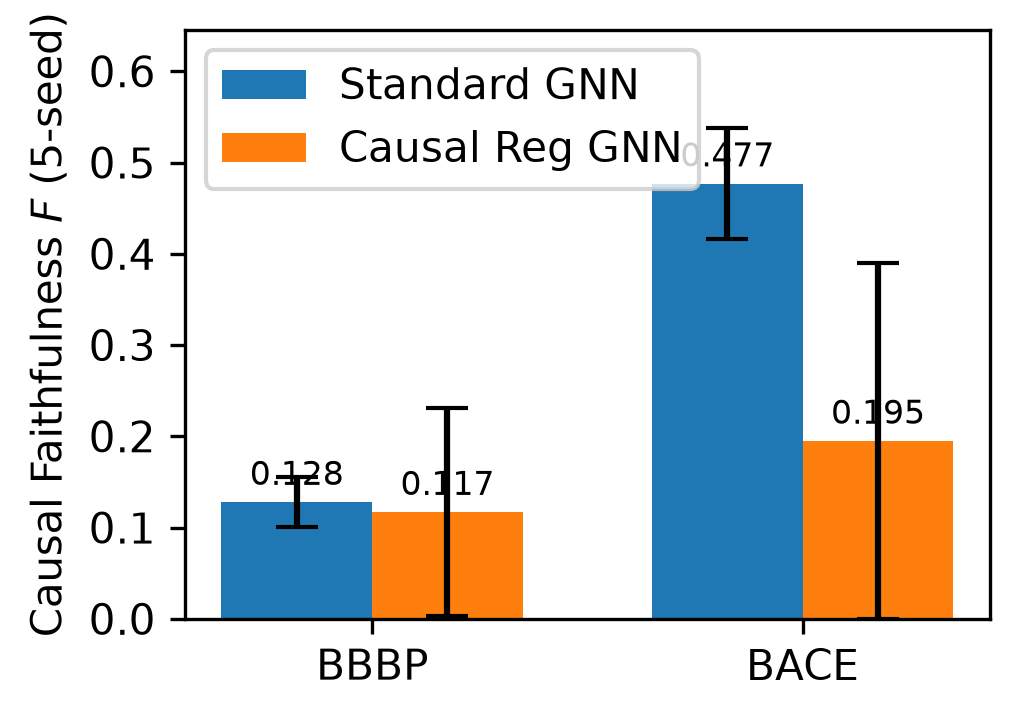
\includegraphics[width=0.78\columnwidth]{figures/causal_faithfulness_5seed.png}
\caption{Five-seed counterfactual consistency (CCS; fraction of toxicophore removals that drop the prediction by $\geq 0.1$). BBBP: standard GNN and causal-regularized GNN are statistically indistinguishable ($\Fcausalstd\pm\Fcausalstdsd$ vs $\Fcausalreg\pm\Fcausalregsd$, Welch $p=0.83$); the regularizer adds instability, not consistency. On BACE the regularizer is significantly \emph{worse} than baseline ($\BACEcausalstd\pm\BACEcausalstdsd$ vs $\BACEcausalreg\pm\BACEcausalregsd$, Welch $p=0.029$). Error bars = sample std. See Table~\ref{tab:faith} for the full cross-dataset comparison.}
\label{fig:faith}
\end{figure}

\section{Discussion}
The practical implication is that GNN toxicity predictions should not be trusted on the basis of their highlighted substructures alone: under the evaluated conditions, standard empirical risk minimization on this architecture does not induce alignment between attributed substructures and the model's decision boundary, and counterfactual removal of the annotated substructure failed to reduce predicted toxicity in the majority of valid cases. Faithfulness tooling must therefore be verified, not assumed. Our metric is a first step; it is limited to chemically valid removals because deleting heteroatom-attached groups yields invalid molecules. We report the metric's behaviour transparently.

A notable cross-dataset difference is that the \emph{untrained} GNN is already far more causally faithful on BACE ($0.477\pm0.061$) than on BBBP ($0.128\pm0.027$), a $\approx 3.7\times$ gap in the baseline itself. This is not contradictory: BACE is a larger, more class-balanced dataset in which the probed substructures (halogens, nitro, epoxide) are more systematically linked to the $\beta$-secretase-inhibition label, so removing one more often drops the prediction; BBBP's blood--brain-barrier endpoint is driven by a broader, less localizable set of physicochemical properties, weakening any single-substructure causal signal. The harmful effect of the regularizer on BACE therefore means it degrades an already-present signal rather than failing to create one.

A second implication concerns the regularizer literature: a conceptually simple causal prior (mask toxicophores, penalize predictions that survive their removal) did not produce more consistent models and introduced predictive instability. This suggests that toxicophore presence is only weakly aligned with the saliency the GNN actually uses, and that more structured causal objectives (e.g., invariant or interventional objectives) are needed---an open direction we document rather than over-claim.

\subsection*{Implications for Future GNN Explainability Research}
Our negative result carries three direct implications for the community.
First, faithfulness of GNN explanations cannot be assumed from architectural
choice alone---even architectures with strong expressive power (GIN, GINE)
do not, under standard ERM, learn decision boundaries aligned with
chemically-interpretable substructures. Second, the metric-disagreement
between our structural counterfactual (CCS) and the gradient-deletion score
demonstrates that faithfulness claims are method-specific and
not interchangeable; future work should report multiple complementary
faithfulness probes rather than any single score. Third, the failure of a
simple margin-based causal regularizer to improve consistency---while
degrading predictive stability---suggests that inducing causal alignment
in GNNs may require more principled objectives, such as invariant risk
minimization~\cite{arjovsky2019invariant} or causal-graph-aware message
passing. Our findings suggest caution when LLM-generated explanations are
layered on models whose underlying explanations have not themselves been
causally verified.

\section{Limitations}
\textbf{Single-model family.} We evaluate one GINE architecture as a minimal expressive MPNN without massive pretraining confounders; while the protocol is model-agnostic, evaluating Graph Convolutional Networks (GCN), Graph Attention Networks (GAT), and pretrained Graph Transformers (Mole-BERT, GraphMAE) is an essential direction for future work. \textbf{Chemical-validity of counterfactuals.} Automatic removal cannot produce valid molecules for many functional groups, so faithfulness is measured over the 68.1\% valid subset and a conservative toxicophore vocabulary; broader alert coverage is future work. \textbf{Single-seed ChemProp.} Computational constraints prevented multi-seed reproduction of the ChemProp baseline; we report the canonical single-seed ChemProp baseline from MoleculeNet as a reference point and acknowledge that a single-seed comparison lacks variance estimation for formal significance testing. \textbf{ClinTox not included.} We trained BBBP, BACE, and TOX21 only; ClinTox (ChemProp \ChemClin) is left for future work as it requires separate multi-task calibration and does not affect the faithfulness conclusions. \textbf{LLM narrative generation not evaluated.} The original protocol's LLM-based rationale step requires an external API the present environment cannot run; we scope this paper to GNN-level causal verification, which is fully reproducible here, and treat language-model explanation as a downstream direction.

\section{Reproducibility}
All numbers derive from committed result files under \texttt{benchmark\_results/} (per-seed AUROC JSONs, faithfulness seed JSONs, \texttt{VALIDATION\_LOG.md}, \texttt{ABLATION\_TABLE.md}). The faithfulness harness (\texttt{run\_real\_faithfulness.py}) accepts \texttt{--ckpt}/\texttt{--out}/\texttt{--dataset} and reproduces every reported figure, including the threshold-sensitivity table; training uses \texttt{train\_real\_graph.py} with \texttt{--causal\_reg}.

\section{Conclusion}
We showed that a competitive GINE toxicity model does not, by default, induce counterfactual consistency, that a simple margin-based masking regularizer only adds instability (and on BACE reduces consistency), and that reporting this honestly---with a sanity-checked metric, a random-removal null, a second faithfulness measure, confidence intervals, threshold sensitivity, and documented tooling limits---is more useful than an unverified faithfulness headline.

\bibliographystyle{cas-model2-names}
\bibliography{references}

\end{document}